\section{はじめに}

% \begin{itemize}
%   \item インフォメーションダッシュボード ⇒ 情報ダッシュボード の方がいいかも
%   \item わかるらんどの思想を述べる
%   \item 消去性コンピューティングについて\cite{kurihara2016}
% \end{itemize}

ワイヤレスネットワークや小型計算機の普及による
IoT社会が到来しつある現在、
人々は大量のリアルタイム情報や通知やメッセージなどに圧倒されている。
%
多くの情報を人間が理解しやすくするため、
以下のような視覚化手法が利用されている。

\vspace{3mm}

\begin{figure}[b]
\centering\fbox{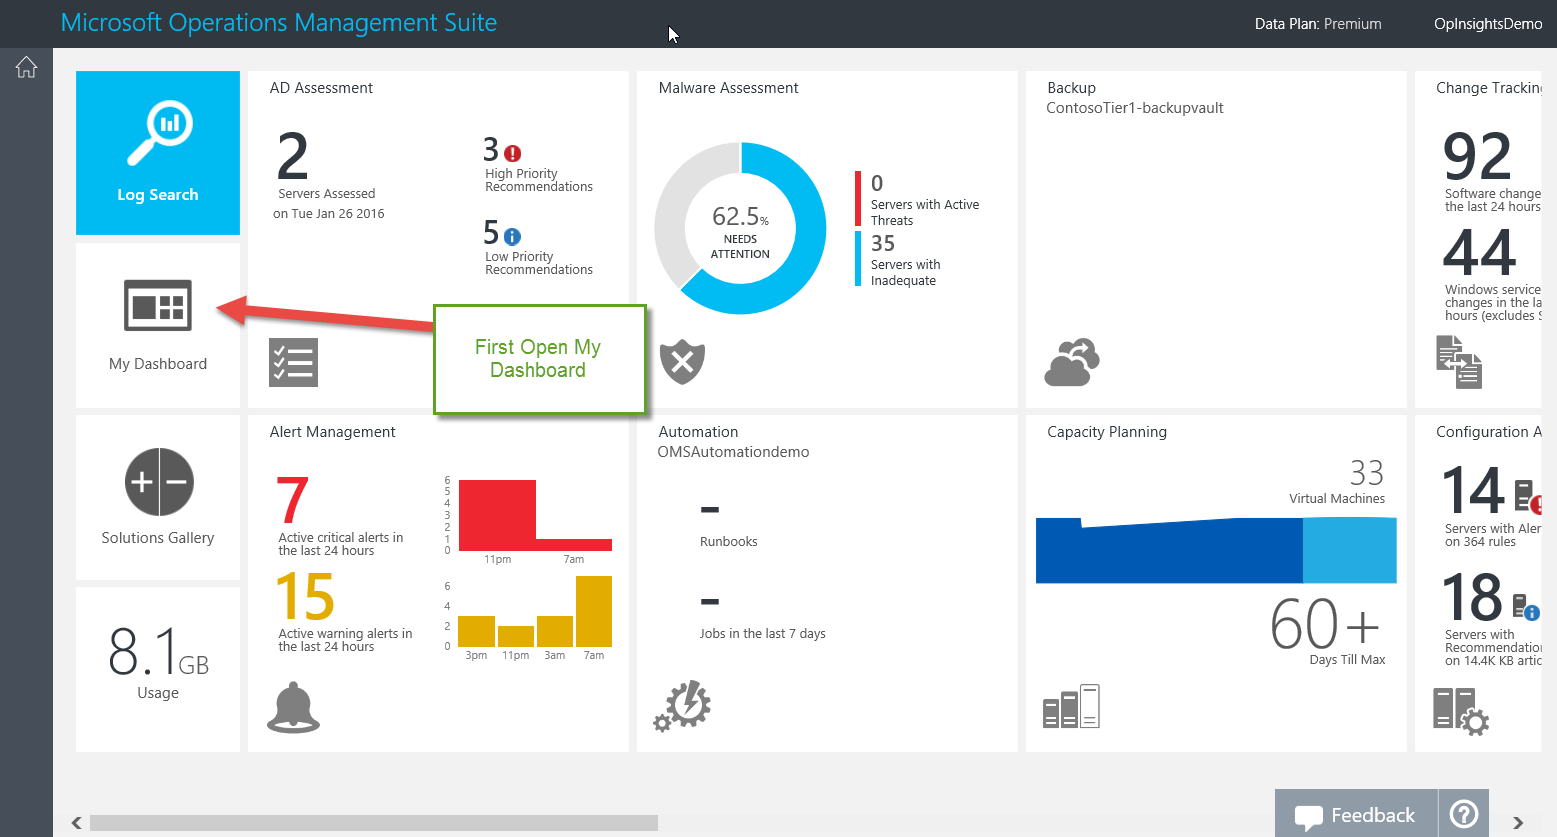
\includegraphics[width=7cm]{images/azure.png}}
\caption{Microsoft Azureの情報ダッシュボード}
\label{azure}
\end{figure}

\paragraph*{情報ダッシュボード}

情報ダッシュボード\cite{few}は、
複数のリアルタイム情報をタイル状に並べて表示することによって
多くの情報をわかりやすく視覚化するシステムである。
たとえばWindowsのスタート画面(図\ref{azure})の情報ダッシュボードには
天気予報や株価のようなリアルタイム情報を表示可能である。

%インフォメーションダッシュボード(図\ref{azure})は、
%単一の画面に複数のリアルタイム情報をタイル状に並べて表示するものだ。
%インフォメーションダッシュボードはセンサの値や株価など常に値が変化していくものをたくさん並べて、
%ひと目で把握するのに非常に便利なインタフェースである。
%しかし、表示領域が限られているため、長いテキストを表示するには適していない。

% ひと目で把握するのに非常に便利なインタフェースである。
% しかし、表示領域が限られているため、長いテキストを表示するには適していない。

% 現在我々は多くの情報の中で生活している (????)。
% SNSやニュースなどはインターネット上に流れていて簡単に見ることができるが、
% 誰が今何を考えているのか、どこにいて何をしているのかといった情報も知りたいことがある。
% それを実現するためにはありとあらゆる情報を簡単にアウトプットできて、それらを見ることが
% できるシステムが必要である。

% 現在ある、情報を見るためのインタフェースの工夫として、
% \begin{itemize}
% \item タイムライン表示
% \item インフォメーションダッシュボード
% \item スタンプ
% \end{itemize}
% の3つを紹介する。

\vspace{2mm}
\paragraph*{タイムライン表示}

Twitter, Facebook, LINEのような
近年のコミュニケーションシステムでは、
投稿を時系列に並べて表示する
「タイムライン表示」(図\ref{twitter})が広く利用されている。
%
タイムライン表示はリアルタイムに更新され、
時間順に情報を見るのには便利であるが、
投稿の多いユーザの記事ばかりが目立ちがちだし、
古い投稿がすぐに見えなくなってしまうという問題がある。

\begin{figure}[H]
\centering\fbox{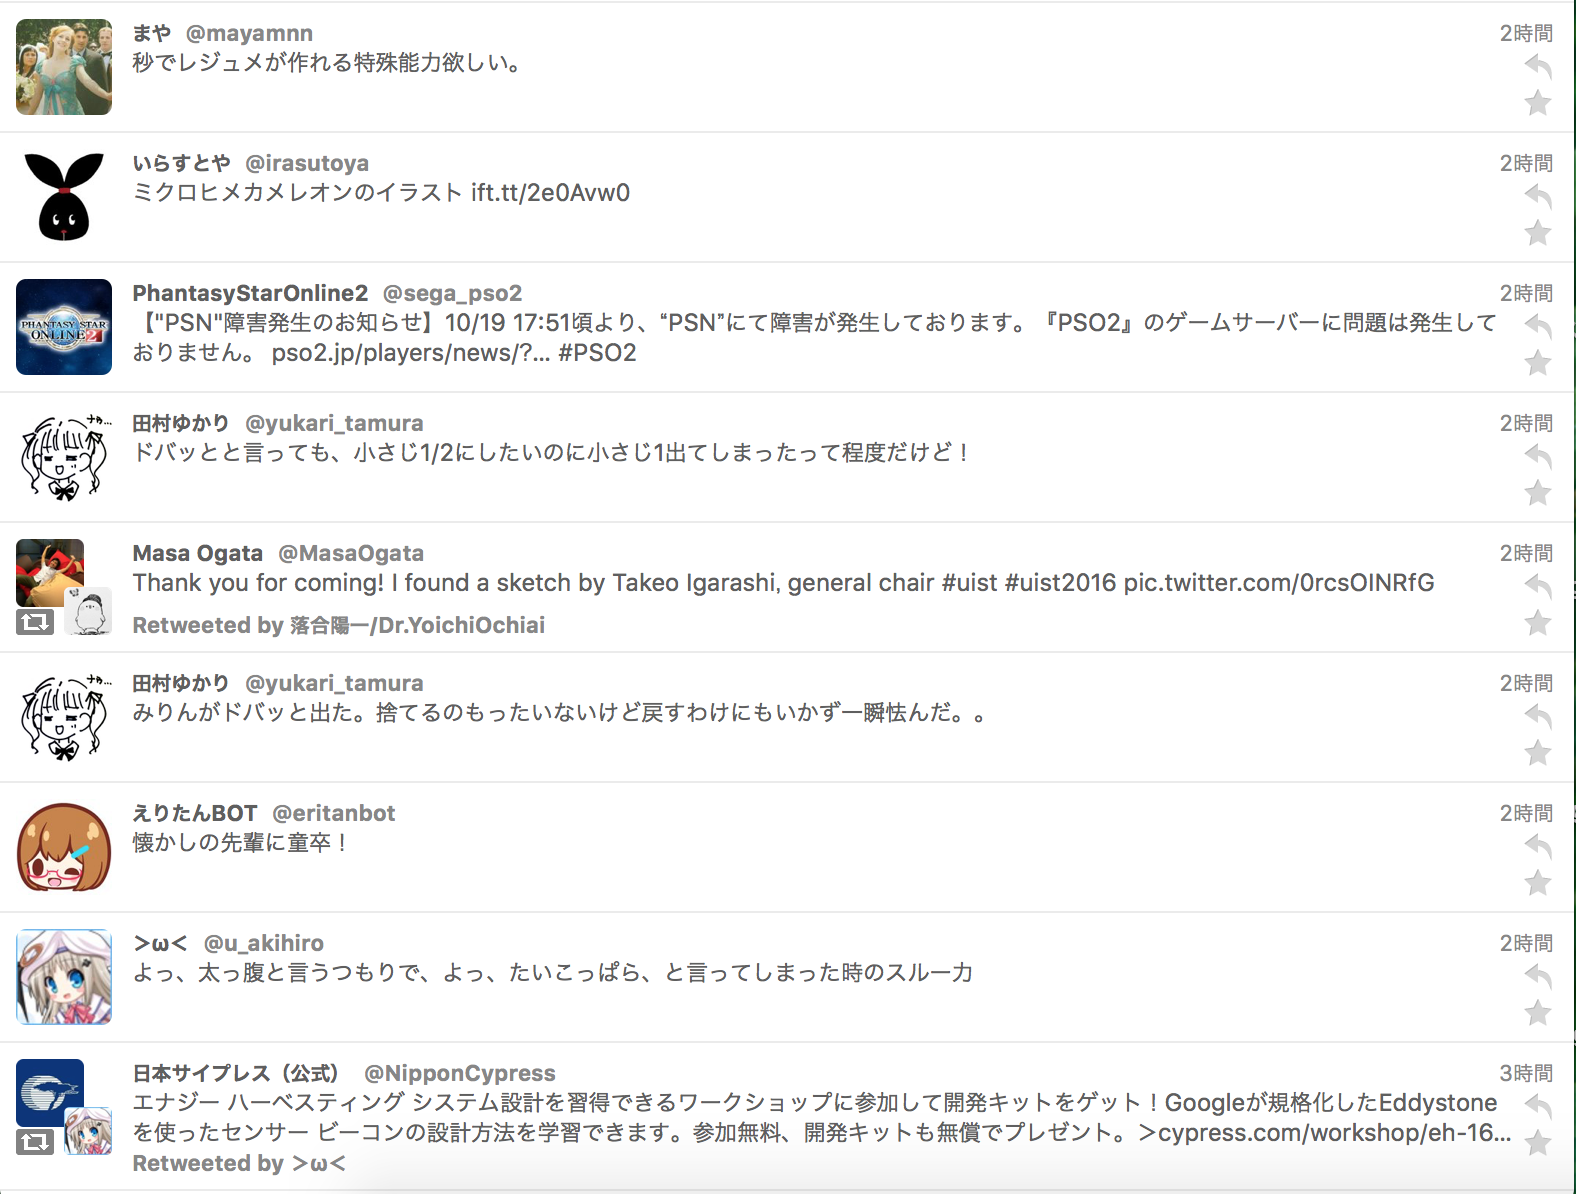
\includegraphics[width=7cm]{images/twitter.png}}
\caption{Twitterのタイムライン}
\label{twitter}
\end{figure}

\vspace{1mm}
\paragraph*{スタンプ}

リアルタイムに流れていくタイムライン表示の中で情報を目立たせたいとき、
近年は「スタンプ」と呼ばれるピクトグラムが利用されることが多くなってきた(図\ref{stamp})。

スタンプはテキストで記述するのが難しい表現や感情を伝えたり、
テキストを考えて入力するよりも速くて簡単であったりすることから、
近年LINEやFacebookメッセンジャー、オンラインゲームなどで広く利用されている。

\begin{figure}[H]
\centering\fbox{
\includegraphics[width=4cm]{images/linestamp.png}}
\caption{LINEのスタンプの例}
\label{linestump}
\end{figure}

\vspace{3mm}
そこで、このスタンプをダッシュボードのセルに表示することで、
ダッシュボードとスタンプベースのコミュニケーションを組み合わせた視覚化システム
『わかるらんど』を開発した。
『わかるらんど』は単純なアーキテクチャで、人の感情や現在の状況、
IoT機器の情報などをリアルタイムに視覚化するシステムで、
非常に汎用なダッシュボードとして利用することができる。




